\paragraph{Упаковка моделей}

Финальным шагом обработки информационных моделей является упаковка.
Для этого был выбран механизм фреймворка Unity называющийся AssetBundle.
AssetBundle это архив, содержащий не скриптовые ресурсы,
например модели или текстуры, который можно динамически загружать
или выгружать в момент выполнения приложения.
Пакеты могут обладать взаимными зависимостями, например графический материал,
упакованный в один AssetBundle может использовать текстуру,
упакованную в другой AssetBundle (рисунок~\ref{figure:AssetBundleDependency}),
что может сильно уменьшить расход памяти, если таких пакетов
с графическими материалами станет несколько.%
\cite{DocUnity,UnityAssetsResourcesBundles}

\begin{figure}[!htp]
    \centering
    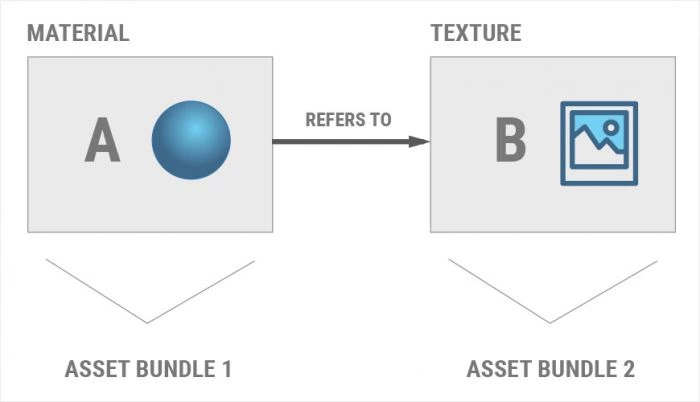
\includegraphics[width=0.8\textwidth]{images/AssetBundleDependency.png}
    \caption{Взаимозависимости ресурсных пакетов.%
    \cite{UnityAssetsResourcesBundles}}
    \label{figure:AssetBundleDependency}
\end{figure}

Помимо этого AssetBundle обладает встроенными механизмами сжатия,
а также механизмами версионности и кеширования,
что позволит эффективнее справляться с модификациями информационной модели.%
\cite{DocUnity,UnityAssetsResourcesBundles}
Создание ресурсных пакетов тоже может быть полностью автоматическим,
что показано на рисунке~\ref{figure:SExportBundles}.

\begin{figure}[!htp]
    \centering
    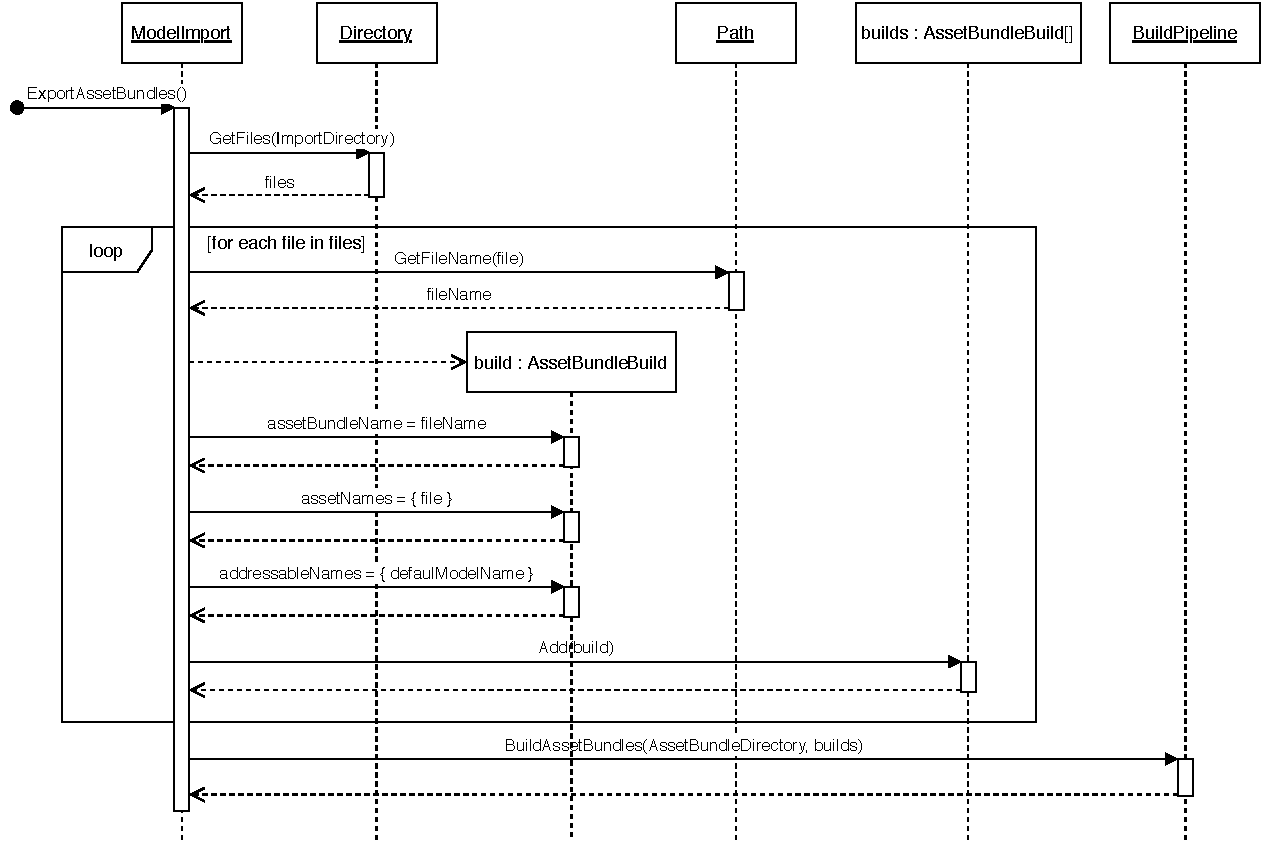
\includegraphics[width=1.0\textwidth]{images/UML-SExportBundles.pdf}
    \caption{Экспорт пакетов}
    \label{figure:SExportBundles}
\end{figure}

Для создания AssetBundle'ов необходимо вызвать соответствующий метод
у класса, отвечающего за программное инициирование сборки проекта Unity
(\emph{BuildPipeline}). В методе необходимо указать конечную директорию,
в которой будут размещены пакеты, а также информацию по каждому создаваемому пакету,
включающую название пакета, перечень ресурсов, включаемых в пакет,
а также соответствующие ресурсам имена, используемые при извлечении
ресурсов во время работы приложения.\cite{DocUnity,UnityAssetsResourcesBundles}
